%====================================================================
\backupbegin
%====================================================================

%====================================================================
\frame{\frametitle{Adaptive step size}

  \paragraph{Conditional ESS:} efficiency of sample $\Ecal$ from $q$ for distribution $p$
  $$
  cESS(\Ecal; q, p) = \frac{M \left(\sum_m W^m a^m\right)^2}{\sum_m W^m (a^m)^2}, 
  \qquad a^m = \frac{p(U^m)}{q(U^m)}
  $$
  \ra Step 1: find next $q_h$ s.t. sample $\Ecal_{h-1}$ is reasonably efficient.
  
%   \bigskip \bigskip \bigskip \pause
%   \paragraph{ESS:} intrinsic efficiency of a sample 
%   $$
%   ESS(\{(U^m, w^m)\}) = \frac{M \left(\sum_m w^m\right)^2}{\sum_m (w^m)^2}
%   $$
%   \ra Step 1c: resample if to few particles actually contribute
  
  \bigskip \bigskip \pause
  Update formula of the weights
  $$
  cESS(\Ecal_{h-1}; q_{h-1}, q_h) 
  = 
  \frac
  {M \left[\sum_m W_{h-1}^m \; (\emphase{r^m_{h-1}})^{\rho_h -\rho_{h-1}}\right]^2}
  {\sum_m W_{h-1}^m \; (\emphase{r^m_{h-1}})^{2\rho_h - 2\rho_{h-1}}}
  $$
  \ra can be computed for any $\rho_h$ \emphase{before sampling}.
  
  \bigskip
  \ra $\rho_h$ tuned to meet $\tau_1$, which controls the step size $\rho_h - \rho_{h-1}$ (and $H$)
}

%====================================================================
\frame{\frametitle{Marginal likelihood}

  Denote
  $$
  \gamma_h(U) = \pt(U) \alpha(U)^{\rho_h}, 
  \qquad Z_h = \int \gamma_h(U) \d U,
  \qquad q_h = \gamma_h(U) / Z_h
  $$
  
  \bigskip
  The marginal likelihood is given by
  $$
  p(Y) = \int p_0(U) \ell(Y|U) \d U = \int \gamma_H(U) \d U = Z_H
  $$

  \bigskip
  which can be estimated with
  $$
  \widehat{\left(\frac{Z_H}{Z_0}\right)} = \prod_{h=1}^H \widehat{\left(\frac{Z_h}{Z_{h-1}}\right)} 
  \qquad \text{where} \quad
  \widehat{\left(\frac{Z_h}{Z_{h-1}}\right)} = \sum_m W_h^m (\alpha_h^m)^{\rho_h - \rho_{h-1}}
  $$
}
  
%====================================================================
\frame{\frametitle{Residual structure}

  Between group interactions ($\alpha_{k\ell}$) = 'residuals' = not explained by the covariates.

  \pause
  \hspace{-.05\textwidth}
  \begin{tabular}{cc}
    \begin{tabular}{p{.4\textwidth}}
      \paragraph{'Graphon' representation.} \refer{LRO17} \\
      Group interactions encoded as
      $$
      \phi: [0, 1]^2 \mapsto \Rbb
      $$
      \begin{itemize}
       \item symmetric\footnote{with increasing marginal $\overline{\phi}(u) = \int \phi(u, v) \d v$ to ensure identifiability.}, 
       \item block-wise constant, 
       \item block width $= \pi_k$
       \item block height $= \alpha_{k\ell}$
      \end{itemize}
    \end{tabular}
    & 
    \begin{tabular}{p{.5\textwidth}}
      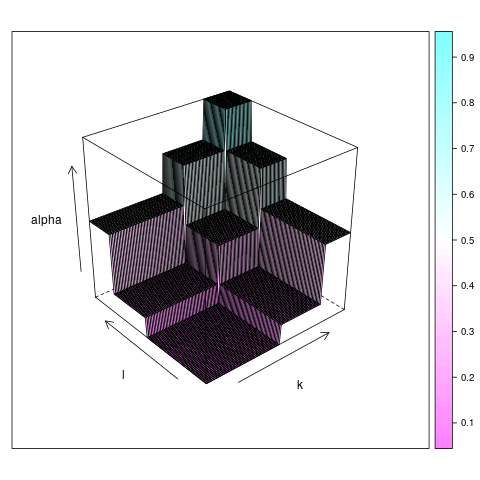
\includegraphics[trim=50 50 50 50, width=.5\textwidth, clip=T]{\fignet/FigGraphon-SBM-graphon-alpha}
    \end{tabular}
  \end{tabular}
  
%   \vspace{-.1\textheight}
  \pause 
  \paragraph{Same representation for all $K$.}
  $
  Y_{ij} | (U_i, U_j) \sim \Pcal\left(\exp(\phi(U_i, U_j) + x_{ij}^\trans \beta \right)
  $
  
  }

%====================================================================
\frame{\frametitle{Tree network residual structure}

%   \vspace{-.2\textheight}
  \hspace{-.04\textwidth}
  \begin{tabular}{cc}
    \begin{tabular}{p{.4\textwidth}}
      \paragraph{Residual graphon.} \\
      Each particle $\theta^m$ provides an estimate of $\phi^m(u, v)$ \\
      ~ \\
      ~ \\
      All estimates can be averaged (over both $m$ and $K$)
    \end{tabular}
    & 
    \pause
%     \hspace{-.05\textwidth}
    \begin{tabular}{p{.5\textwidth}}
    \includegraphics[trim=50 50 50 50, width=.5\textwidth]{\figtree/Tree-all-V10-M5000-graphon}
    \end{tabular}
  \end{tabular}
  
%   \vspace{-.1\textheight}
  \pause
  \paragraph{Interpretation.}
  \begin{itemize}
   \item A remaining individual effect (some species interact more than other in average)
   \item A small fraction of species interact much less than expected.
  \end{itemize}

}
  
%====================================================================
\backupend
%====================================================================

